\documentclass[amsmath,amssymb,notitlepage,11pt]{revtex4-1}
\usepackage{graphicx}
\usepackage{bm}% bold math
\usepackage{multirow}
\usepackage{booktabs}
\usepackage{verbatim}
\usepackage{hyperref}
\hypersetup{pdftex,colorlinks=true,allcolors=blue}
\usepackage{ulem}
%\usepackage[small,compact]{titlesec}
%\usepackage{showkeys}
\addtolength{\textheight}{0.3cm}
\addtolength{\topmargin}{-0.15cm}
\addtolength{\textwidth}{0.4cm}
\addtolength{\hoffset}{-0.2cm}
\begin{document}
\hspace*{11.5cm}

\title{Investigation of EG6 RTPC $z/\theta$ Error}
\author{N. Baltzell}
\affiliation{Argonne National Laboratory}
\date{\today}
\begin{abstract}
There is an obvious and significant error on the recoil vertex measured by the RTPC that varies systematically with the track's polar angle.  This could actually be the result of a corresponding error on the polar angle.  There is also some $z$-dependence to this effect, that, while less significant than the $\theta$-dependence, could help to understand the source of the problem.  Possible causes are considered.%  This writeup serves as documentation of the known facts in hopes that it will help us find the real cause.
\end{abstract}
\maketitle
\tableofcontents
\section{Introduction}
There is a clear error on the RTPC's reconstructed vertex that varies with the polar angle of the track.  This is shown in the bottom left of Fig.~\ref{fig:dzclasrtpc} where the RTPC track's vertex is compared to that of an electron detected in CLAS.
%Since the effect is doubled when we compare two tracks in the RTPC in the same event (right panel of Fig.~\ref{fig:dzclasrtpc}), it must be due to the RTPC.
The doubling of the slope when removing the CLAS track and instead comparing to another good track in the RTPC in the same event (bottom right of Fig.\ref{fig:dzclasrtpc}) suggests that the effect is really due solely to the RTPC.
This was not noticed during calibration, largely because the focus was on $^4$He elastic scattering that covers a small range of recoil angles that happens to be where the effect is small.
\begin{figure}[htbp]\centering
    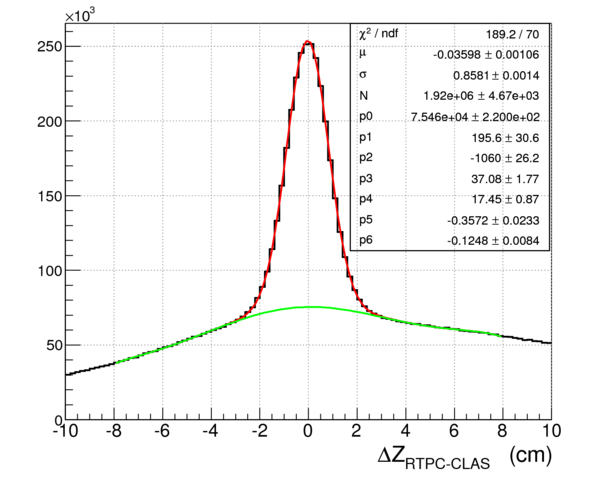
\includegraphics[width=0.49\textwidth]{pics/dvzRTPC-CLAS_small.png}
    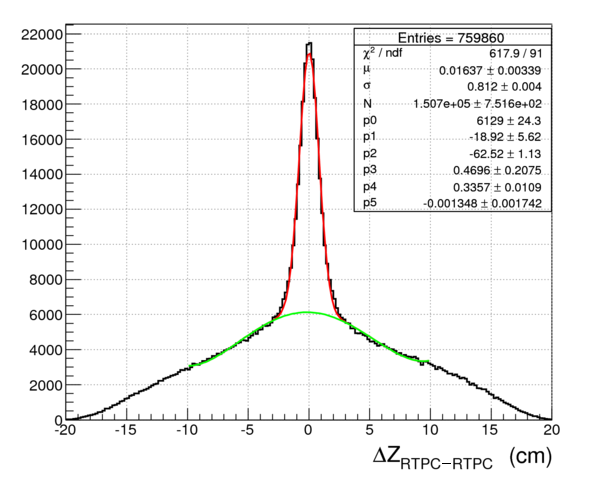
\includegraphics[width=0.49\textwidth]{pics/dvzRTPC-RTPC_small.png}
    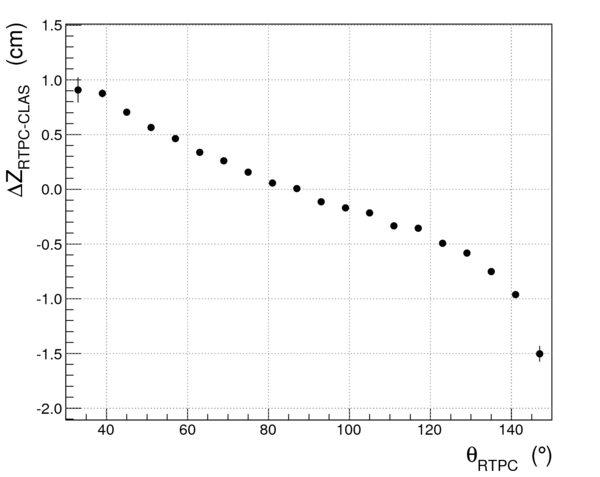
\includegraphics[width=0.49\textwidth]{pics/dvzRTPC-CLAS_vs_theta_small.png}
    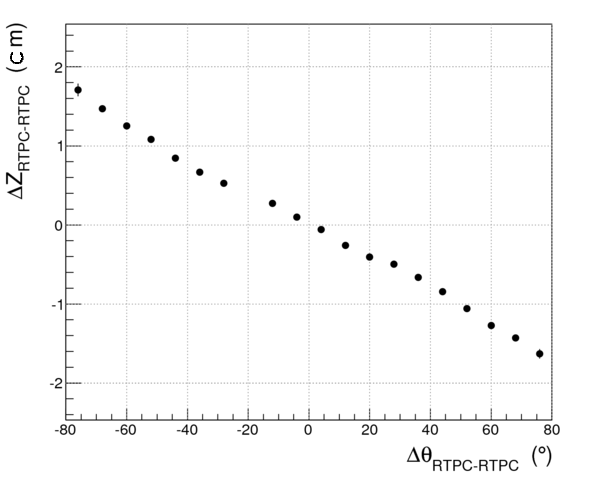
\includegraphics[width=0.49\textwidth]{pics/dvzRTPC-RTPC_vs_dtheta_small2.png}
%    \caption{On left (right) is the RTPC-CLAS (RTPC-RTPC) $z$-vertex difference.  The bottom row is the peak position as a function of RTPC track angle.  That the slope doubles from left to right suggests that the effect in CLAS-RTPC is really due solely to the RTPC.\label{fig:dzclasrtpc}}
    \caption{
    The top row shows the $z$-vertex difference between RTPC tracks and CLAS electrons (left) and two RTPC tracks (right) in the same event.
    The bottom row shows the angular dependence of the peak position.\label{fig:dzclasrtpc}
    %peak position of the RTPC-CLAS $z$-vertex difference as a function of RTPC track polar angle (left).  For two-track events in the RTPC, the peak position of the difference between their vertices as a function of their angle difference (right).\label{fig:dzclasrtpc}
    %That the slope doubles when removing the CLAS track and instead comparing to another track in the RTPC suggests that the effect is really due solely to the RTPC.\label{fig:dzclasrtpc}
    }
\end{figure}

We can measure the error on the vertex over the RTPC's acceptance and correct for it, or similarly apply a multidimensional cut on the vertex difference between the recoil and electron, and thus reduce background under the concidence peak.
However, since the RTPC's vertex is reconstructed directly from its track angle, it is reasonable to suspect there is a corresponding systematic error on the angle.  And the angle measurement affects much more than background/signal ratio; unlike the vertex, it is directly involved in the calculation of physics quantities.

Unfortunately, it is difficult to directly measure from an overly constrained reaction the error on the angle for a significant range of kinematics.  This is due to RTPC and CLAS resolutions, large momentum differences between the two detectors' tracks, and limited kinematic range for any given reaction.  Therefore, it is important to understand the cause of the vertex error.

In this writeup, first the significance of the error on $\theta$ that would create the measured error on $z$-vertex is estimated.  Then possible sources of the error are investigated.
The plots are from a skim of all the data, with the requirement of exactly one electron and at least one neutral calorimeter hit.

\section{Angular Error Prediction}
The relationship between an error on the vertex and angle, {\it assuming full correlation}, is given by the derivative:
\begin{equation}
    \frac{\partial\theta}{\partial z_v} = \frac{\sin^2\theta}{\mathcal{R}}
    \label{eq:dthetadz}
\end{equation}
While this was derived for a straight track, it is also true for a helical path in a solenoid field where curvature is dominantly in the $\hat{\phi}$ direction.
Here $\mathcal{R}$ is the radial distance from the beamline to where the track is measured.
For the purposes of this study, 4.5 cm is assumed, or halfway through the drift region (the cathode is at 3 cm and the GEMs are at 6 cm).

If we {\it assume the error on the vertex is entirely due to an error on $\theta$}, then we can calculate the corresponding error on $\theta$ via: $\delta\theta=\frac{\partial\theta}{\partial z}\delta z$,  where $\delta z$ can be the measured vertex error in the lower left panel of Fig. \ref{fig:dzclasrtpc}.  This results in a significant effect on $\theta$ in Fig. \ref{fig:dtheta1}.

During calibrations using 1.2 GeV beam and elastically scattered $^4$He with an average angle of $78^\circ$, the difference between the measured and expected RTPC angle had a width of $\sim3^\circ$ and was shifted by $+2^\circ$ from zero.  Coincidentally, the prediction in Fig. \ref{fig:dtheta1} suggests a similar $+2.5^\circ$ error on the RTPC angle.  
Coherent $^4$He DVCS is being exclusively reconstructed in 6 GeV EG6 data with measured recoil angles between $50^\circ$ and $70^\circ$.  This prediction in Fig. \ref{fig:dtheta1} implies there could be a $\sim5^\circ$ error at those kinematics, and exclusivity variables are significantly affected by an error of that size.
Clearly it is useful to understand whether the cause of the error on the $z$-vertex is really due to an error on $\theta$.
\begin{figure}[htbp]\centering
    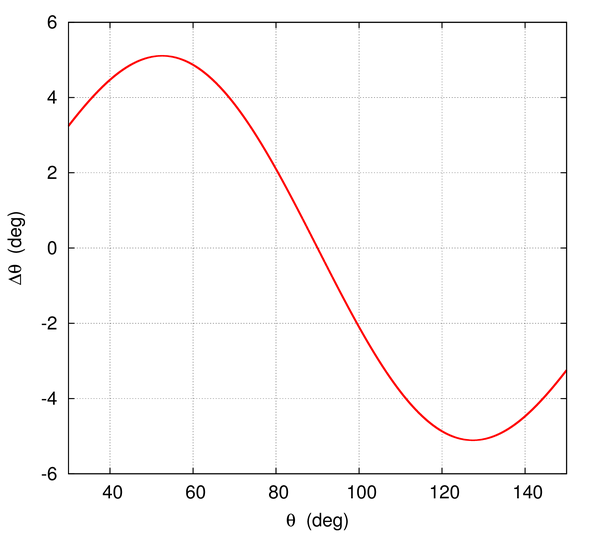
\includegraphics[width=0.49\textwidth]{pics/dtheta1.png}
    \caption{The expected error on $\theta$ assuming the measured error on $z$ originates entirely from an error on $\theta$.  This is the product of Eq. \ref{eq:dthetadz} and a linear parameterization of the lower left plot of Fig. \ref{fig:dzclasrtpc} (which is not accurate for $\left|\theta-90^\circ\right|>40^\circ$).\label{fig:dtheta1}}
\end{figure}
\section{Possible Causes}
While it may be possible to derive corrections empirically from data, with assumptions, or from a full detector simulation, it would be ideal to determine and understand the source of the problem and correct it at its source.
Most of the possible causes thought of so far can be precluded.
%However, an error on the pad pitch is found to exhibit the correct behavior but cannot account for everything.  An unaccounted for effect on the drifts paths could also be involved.

\subsection{Misalignment}
Misalignment has been ruled out as a possible cause because the effect does not exhibit the appropriate behavior when comparing different azimuthal and longitudinal regions of the RTPC.  If misalignment were the culprit, then the effect should not be the same for all the scenarios in Fig. \ref{fig:dz_regions}.  This logical argument should apply to both alignment of the RTPC with respect to the beamline and also the RTPC relative to the solenoid field.  Additionally, RTPC-BEAM misalignment within a reasonably possible range is known to have a negligible effect on reconstruction of $z$-vertex (and $\theta$).% \cite{tpcalign}.
\begin{figure}[htbp]\centering
    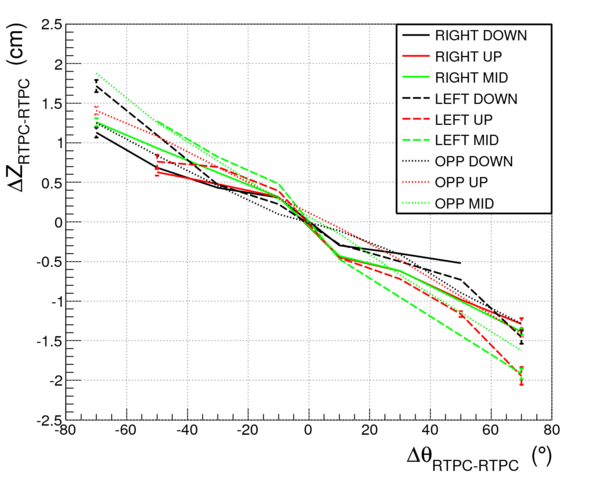
\includegraphics[width=0.49\textwidth]{pics/dz_sides_zpos_small.png}
    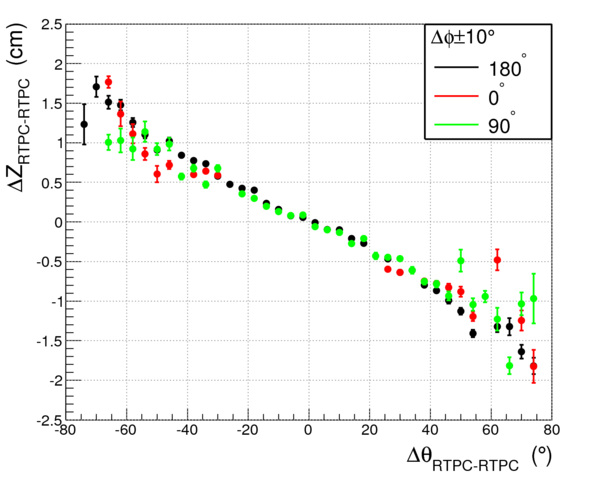
\includegraphics[width=0.49\textwidth]{pics/dz_090180_small.png}
    \caption{The same $\Delta Z$ dependence from the lower right panel of Fig. \ref{fig:dzclasrtpc} but divided into different track geometries.  On left is for different vertex positions (upstream, midstream, and downstream) and different RTPC halves for the two tracks (both right, both left, and opposite).  On right is separated by the azimuthal angle difference of the two tracks. \label{fig:dz_regions}}
\end{figure}
\subsection{Energy Loss}
Energy loss results in an increase in curvature as the track loses energy, particularly in the target wall.  This could affect the validity of the helix fit, especially with a beamline constraint.  However, this seems a doubtful cause since the observed effect increases with momentum as shown in Fig. \ref{fig:dz_mom}.
\begin{figure}[htbp]\centering
    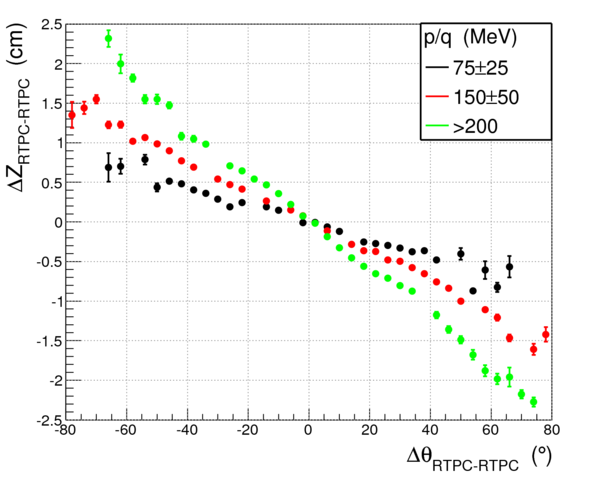
\includegraphics[width=0.49\textwidth]{pics/dzdthe_pbins_small.png}
    \caption{The same as Fig.\ref{fig:dz_regions}, but now separated by track curvature in the drift region ($p/q$).\label{fig:dz_mom}}
\end{figure}
\subsection{Magnetic Field Error}
An error on measurement of the recoil track due to inaccuracy of the solenoid field should decrease with momentum.  However, the opposite behavior is found in Fig. \ref{fig:dz_mom}: the effect increases with momentum.  Furthermore, Fig. \ref{fig:dz_theta_z.png} shows there is another dependence on $z$ that, while smaller than that on $\theta$, is largely independent of $\theta$.
In particular, tracks that pass through the drift region near $z=0$ in the center of the RTPC, where the longitudinal component of the field should be most uniform, and the radial componenet minimial (see field map in Fig. \ref{fig:field}), still have the same $\theta$-dependence.  And tracks at 90$^\circ$ have a $z$-dependence even near the very center of the RTPC.  Also, previous GEANT4 studies showed that there is no significant deviation of the track's angle between the vertex and the drift region.
\begin{figure}[htbp]\centering
    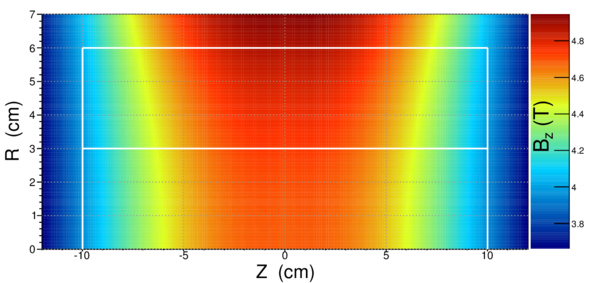
\includegraphics[width=0.49\textwidth]{pics/saclay5_longitudinal_small.png}
    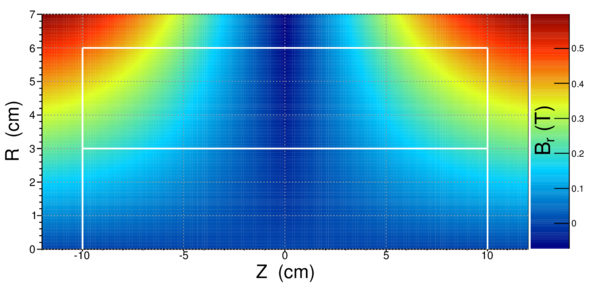
\includegraphics[width=0.49\textwidth]{pics/saclay5_radial_small.png}
    \caption{The longitudinal (left) and radial (right) components ($\hat{z}$ and $\hat{\rho}$ in cylindrical coordinates) of the solenoid magnetic field map (color scale is Tesla, but different range for left/right).  The vertical white lines represent the upstream and downstream ends of the RTPC, and the upper rectangle is the drift region.\label{fig:field}}
\end{figure}
\begin{figure}[htbp]\centering
    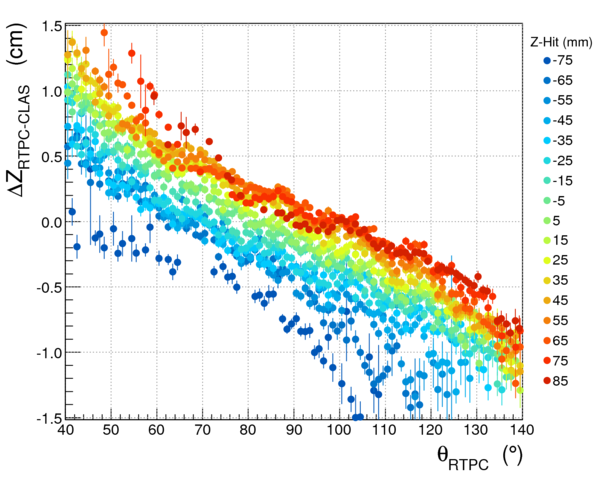
\includegraphics[width=0.49\textwidth]{pics/dz_theta_zhit_fid_A_small.png}
    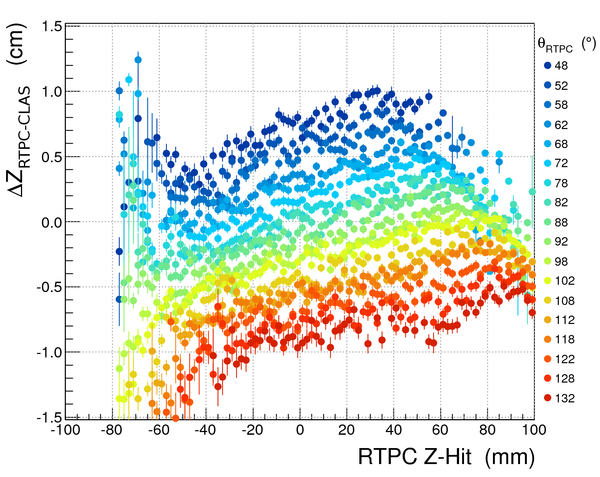
\includegraphics[width=0.49\textwidth]{pics/dz_theta_zhit_fid_B_small.png}
    \caption{A $z$-dependence becomes clear when looking in narrow angular ranges.  The left plot is the same as the bottom left panel of Fig. \ref{fig:dzclasrtpc}, but separated into colors by the average $z$-position of the track as it transverses the drift region.  The right plot just swaps the $x$-axis and colors.\label{fig:dz_theta_z.png}}
\end{figure}
\subsection{Changes in Calibration}
Another hypothesis is we are seeing some effect due to changes in the drift paths calibration over the course of the EG6 run period after the early calibration data.  However, the $\theta$-dependence of $\Delta Z$ is quite constant over time, as is shown in Fig. \ref{fig:dz_theta_runs}.
\begin{figure}[htbp]\centering
    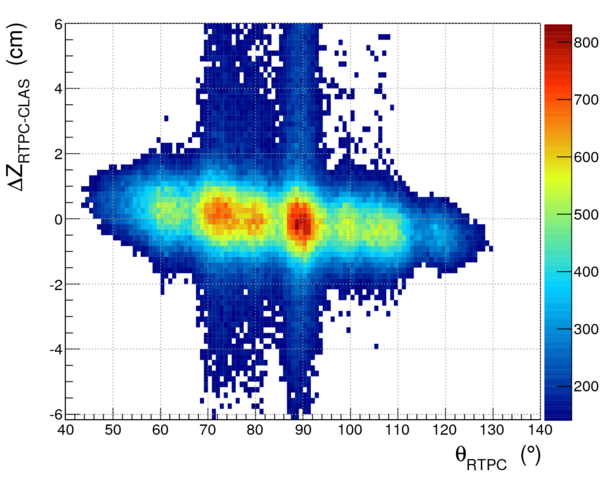
\includegraphics[width=0.49\textwidth]{pics/dztheta_a_small.png}
    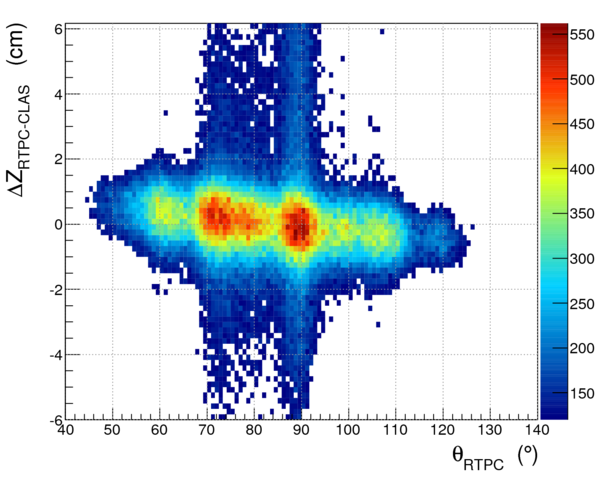
\includegraphics[width=0.49\textwidth]{pics/dztheta_c_small.png}
    \caption{RTPC's $\theta$-dependence of $\Delta Z$ for early (left) and late (right) data in the EG6 run period.  The run ranges are 61510-61608 and 61774-61843.\label{fig:dz_theta_runs}}
\end{figure}

\subsection{Reconstruction Technique}
An error in the logic of the reconstruction algorithm, or not accounting for some physical effect, is a possibility.  However, the $\theta$-dependence is absent in simulations using the same helix fit and reconstruction technique in a different detector.  In the RTPC simulation without drift paths (fitting only to GEANT4's tracking points), the effect is also absent.  Study of the effect of drift paths and discrete pads should be done with the full simulation.%  This could involve unaccounted effects due to the magnetic field on the drift paths.
\subsection{Pad Pitch}
Another possible cause is a difference between the actual pad pitch and that used in the reconstruction code.  Of course, the pad pitch on the real RTPC's GEMs will also be measured, but the analysis in the next section should give an idea of what the effect of such an error would be and whether it can describe the data.

%Are there any other causes that could create a linear $z$-dependence of vertex reconstruction for tracks at 90$^\circ$?

\section{Effect of Incorrect Pad Size}\label{sec:padpitch}
One hypothesis is that the pad size used in the reconstruction may not be the actual pad size of the real RTPC's GEMs.  The effect of such an error can be studied with simple geometrical arguments.  Figure \ref{fig:diagram} illustrates the geometry and variables used in this analysis and shows two GEMs with different pad pitches, $p$.  The position where the two configurations coincide (where they have the same pad at the same $z$-position) is $Z_0$.
\begin{figure}[htbp]\centering
%    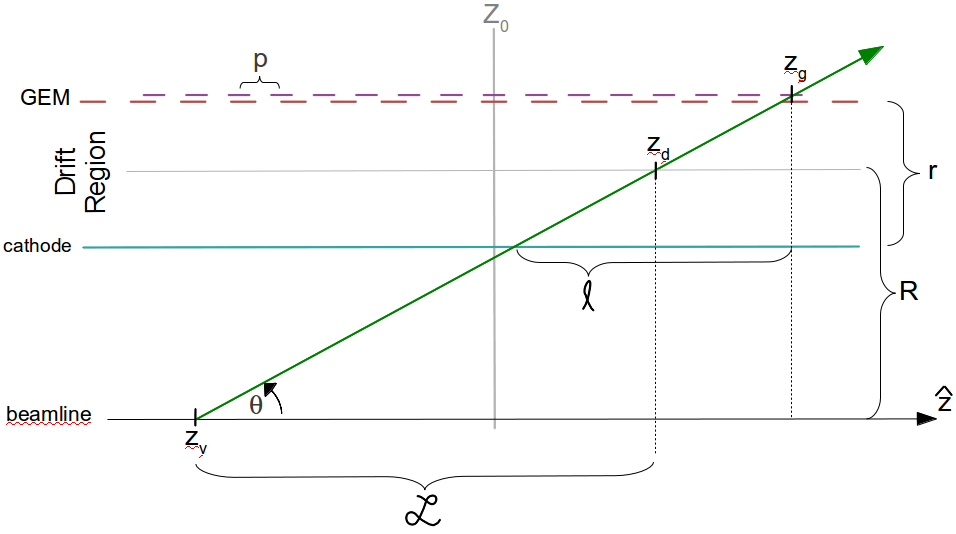
\includegraphics[width=17cm]{pics/diagramA.png}
%    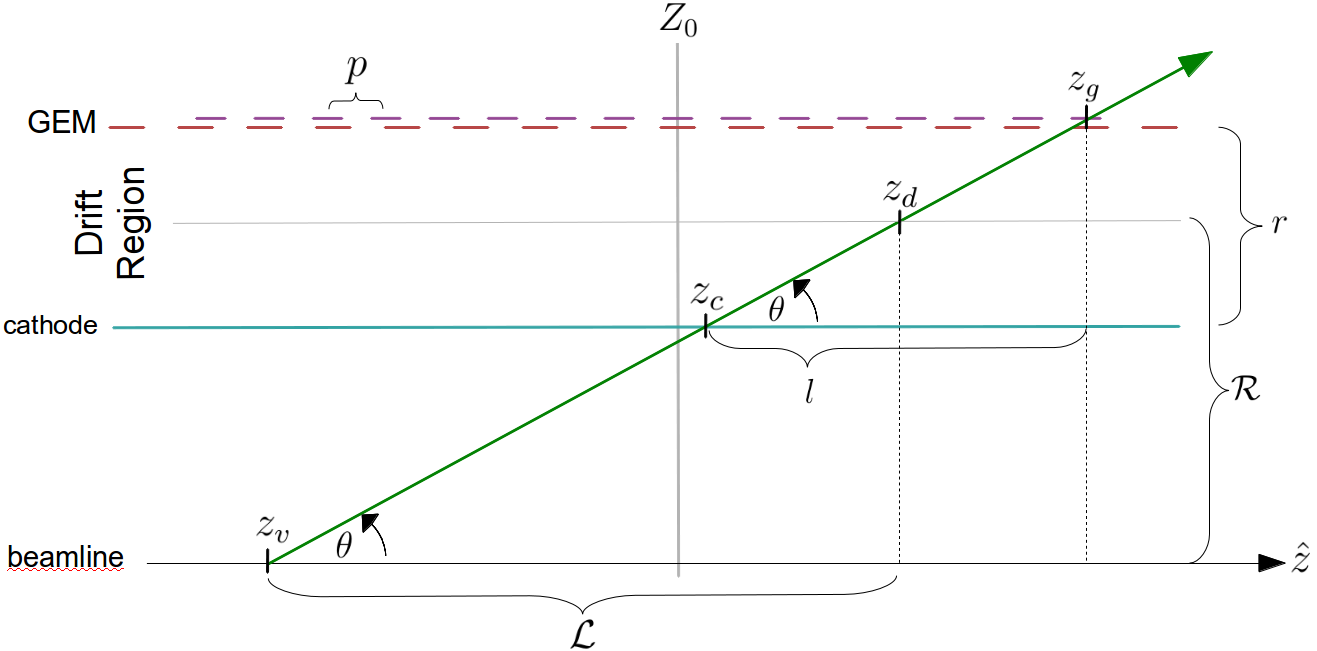
\includegraphics[width=\textwidth]{pics/diagramB.png}
    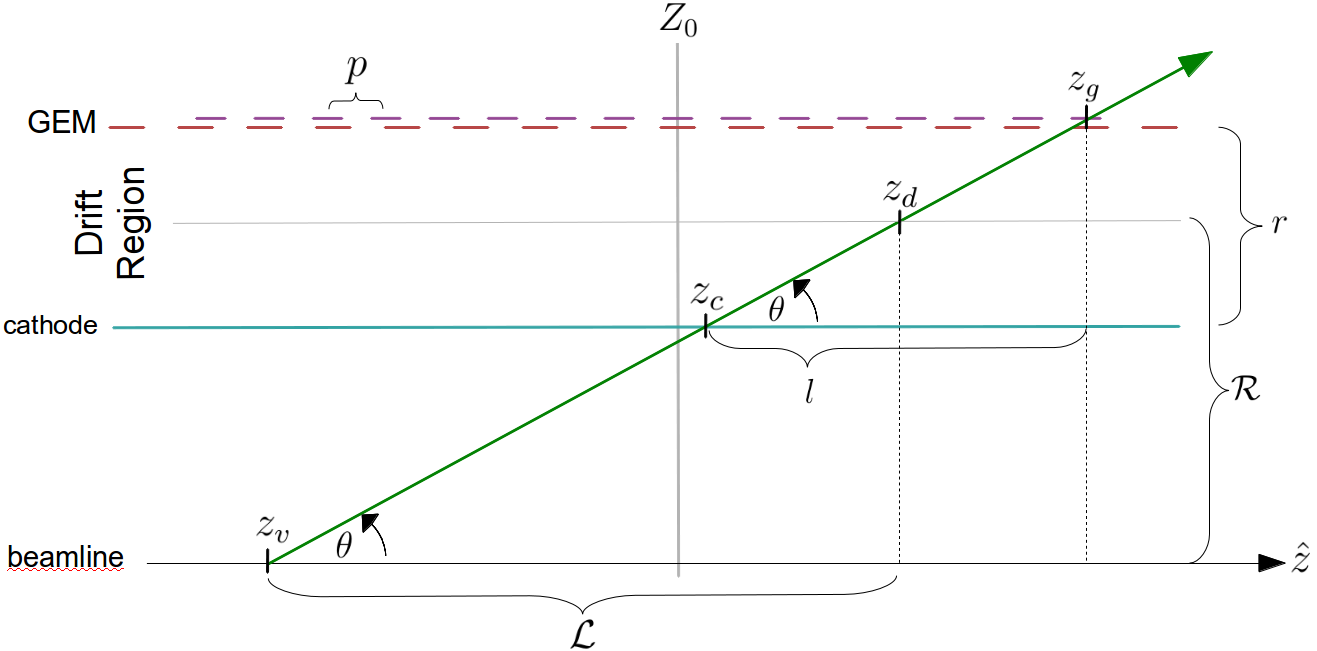
\includegraphics[width=14cm]{pics/diagramB.png}
    \caption{The RTPC tracking geometry for a straight track shown by the green arrow.  The $z$-vertex of the track is $z_v$, and its polar angle is $\theta$.\label{fig:diagram}}
\end{figure}
\subsection{Expected Error}\label{sec:geopitch}
The method of reconstructing the $z$-vertex, denoted as $z_v$, starts with a helix fit to the observed track in the drift region.  This basically gives a measurement of the position of the track in the drift region, the midpoint of which is denoted as $z_d$, and the polar angle of the track, $\theta$. From there, the  angle is used to extrapolate back to the point on the beamline, $v_z$, where the track originated:
\begin{equation}
    z_v = z_d - \mathcal{L}(\theta).
    \label{}
\end{equation}
\subsubsection{Method 1}
The error on the vertex due to error on pitch can then be written:
\begin{equation}
    \delta v_z = \frac{\partial z_d}{\partial p}\delta p - \frac{\partial \mathcal{L}(\theta)}{\partial p}\delta p.
    \label{eq:dvz}
\end{equation}
The first term in Eq. \ref{eq:dvz} is a shift that depends only on the longitudinal position of the track when it crosses the drift region and not directly on the track angle.  Its derivative is linear in $z_d$ and is zero when $z_d=Z_0$:
\begin{equation}
    \frac{\partial z_d}{\partial p} = \frac{z_d-Z_0}{p} = \frac{z_v-Z_0+\mathcal{R}/\tan\theta}{p}.
    \label{}
\end{equation}
The second term in Eq. \ref{eq:dvz} depends only on the angle of the track and not directly on its longitudinal position.  It can be interpreted as a (de)compression of $l$ when the pitch is (increased) decreased.  Its derivative can be decomposed as:
\begin{equation}
    \frac{\partial\mathcal{L}}{\partial p} = \frac{\partial\mathcal{L}}{\partial\theta}\frac{\partial\theta}{\partial p}.
    \label{}
\end{equation}
With the relationship $\frac{\mathcal{R}}{\mathcal{L}}=\frac{r}{l}=\tan\theta$, 
\begin{equation}
    \frac{\partial\mathcal{L}}{\partial\theta} = \frac{-\mathcal{R}}{\sin^2\theta}\ \ \ \ \ \ \ \ \ \ \ \  
    \frac{\partial\theta}{\partial p} = \frac{-\sin\theta\cos\theta}{p}.
    \label{}
\end{equation}
%and then
%\begin{equation}
%    \frac{\partial\mathcal{L}}{\partial p} = \frac{\mathcal{R}}{p\tan\theta}
%    \label{}
%\end{equation}
Combining everything, the angular dependence cancels, resulting in:
\begin{equation}
    \delta v_z = (z_v-Z_0)\frac{\delta p}{p}.
    \label{eq:dz}
\end{equation}
Or, in terms of $z_d$ instead of $z_v$:
\begin{equation}
    \delta v_z = (z_d-Z_0-\frac{\mathcal{R}}{\tan\theta})\frac{\delta p}{p}.
    \label{eq:dz_angle}
\end{equation}

\subsubsection{Method 2}
For a cross check, let's try a simpler method without any derivatives, just a finite error on $z_v$ due to a pitch error.  The primed coordinates are after changing the pad pitch by $\delta p$.
\begin{equation}
    z_v=z_d-\mathcal{L} \ \ \ \ \ \ \ \ \ \ \ \ \   z_v'=z_d'-\mathcal{L}'
    \label{}
\end{equation}
\begin{equation}
    z_d' = z_d + (z_d-Z_0)\frac{\delta p}{p}\ \ \ \  \ \ \ \ \ \     \mathcal{L}'=(1+\frac{\delta p}{p})\mathcal{L}
    \label{}
\end{equation}
%\begin{equation}
%    \mathcal{L}'=(1+\frac{\delta p}{p})\mathcal{L}
%    \label{}
%\end{equation}
Then:
\begin{equation}
    \delta z_v=z_v-z_v'=(z_d-Z_0-\mathcal{L})\frac{\delta p}{p}
    \label{}
\end{equation}
%And eliminating $z_d$ in favor of $z_v+\mathcal{L}$:
%\begin{equation}
%    \delta v_z=z_v'-z_v=(z_v-Z_0)\frac{\delta p}{p}    
%    \label{}
%\end{equation}
This is identical to result of the previous section (Eq. \ref{eq:dz_angle}).  The same is also achieved by writing everything in terms of two $z$-coordinates in the drift region ($z_g$ and $z_c$, for example) and deriving in terms of those variables.

\subsection{Comparison with Data}
Let's see if an error on the pad pitch can account for the error on $z_v$ found in the real data.
\subsubsection{Tracks at $\theta=90^\circ$}\label{sec:90deg}
Tracks at 90$^\circ$ provide a special case to investigate a pad pitch error.
Figure \ref{fig:zdz_90deg} shows the measured dependence of the RTPC-CLAS vertex difference on $z_v$ for only tracks near $90^\circ$.  If we assume the form of Eq. \ref{eq:dz} explains the data, this gives $Z_0=3.3$ cm and $\frac{\delta p}{p}=+0.055$ based upon a linear fit.
So a 5.5\% error (0.27 mm) on the pad size is sufficient to explain the $z$-dependence of the RTPC-CLAS vertex difference for RTPC tracks near $90^\circ$.  
\begin{figure}[htbp]\centering
    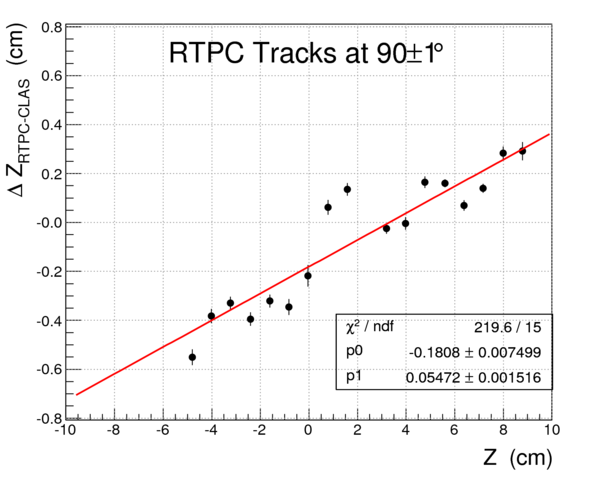
\includegraphics[width=0.49\textwidth]{pics/zdz_90deg_fit_small.png}
    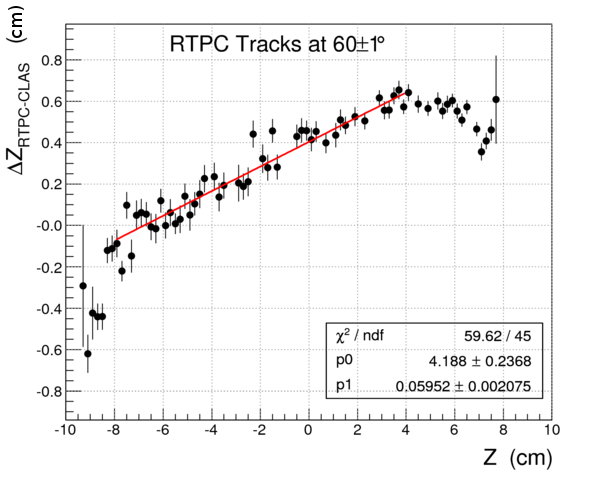
\includegraphics[width=0.49\textwidth]{pics/zdz_60deg_fit_small.png}
    \caption{The peak position of the RTPC-CLAS vertex difference for RTPC tracks near $90^\circ$ (left) as a function of the vertex position in RTPC coordinates (zero is the center of the RTPC).  Tracks near $60^\circ$ (right) give a very similar slope ($\frac{\delta p}{p}$), but require a different $Z_0$ in Eq. \ref{eq:dz}.\label{fig:zdz_90deg}}
\end{figure}
\subsubsection{Tracks Transversing the Center of the Drift Region}\label{sec:z0}
Another special case that may allow simple interpertaion is when the track passes through a localized part of the drift region.  The longidutinal center of the RTPC is of particular interest because there the longitudinal field is most uniform and the transverse field is minimized.

Tracks whose midpoint in the drift region is near $z=0$ is shown in Fig. \ref{fig:thetadz_0cm}.  
Here the fit is using Eq. \ref{eq:dz_angle}, and the data appears to have its $\frac{1}{\tan\theta}$ shape.  However, the fit gives a 16\% error on pitch (2$^{nd}$ fit parameter) to describe the data.  This is in disagreement by a factor of 3 with the 5.5\% from the $z$-dependent fit of the previous section.
\begin{figure}[htbp]\centering
    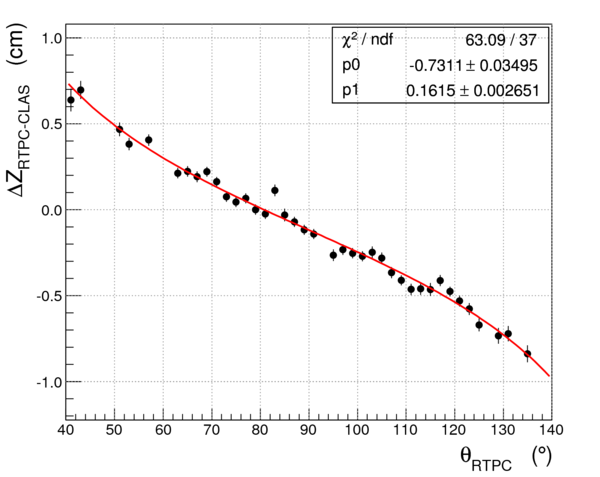
\includegraphics[width=0.49\textwidth]{pics/dztheta_zhit0_fit_small.png}
    \caption{The error on the $z$-vertex for tracks which pass through the center of the drift region ($z_d\sim0$).\label{fig:thetadz_0cm}}
\end{figure}
\subsubsection{Tracks Everywhere}
Based upon the simple geometrical calculation of Sec. \ref{sec:geopitch}, an error on the pad pitch cannot account for every effect we see for $\Delta z$ in Sec. \ref{sec:90deg} and \ref{sec:z0}.  It is possibly just coincidence that the predicted linear $z$-dependence and $\frac{1}{\tan\theta}$-dependence fits the data.  

Nevertheless, it may still be useful to see what effect the corrections from the previous sections would have.  Assuming the result of \ref{sec:90deg}, with 5.5\% $\frac{\delta p}{p}$ and $Z_0=3$ cm, the $z$-dependence is largely removed in the right panel of Fig. \ref{fig:dz_theta_z_corr}.  However, when the $z$-position in the drift region is very near either end of the RTPC, a discrepancy becomes more obvious.  This could correspond with a magnetic field effect on the drift paths where the transverse field is largest.
\begin{figure}[htbp]\centering
    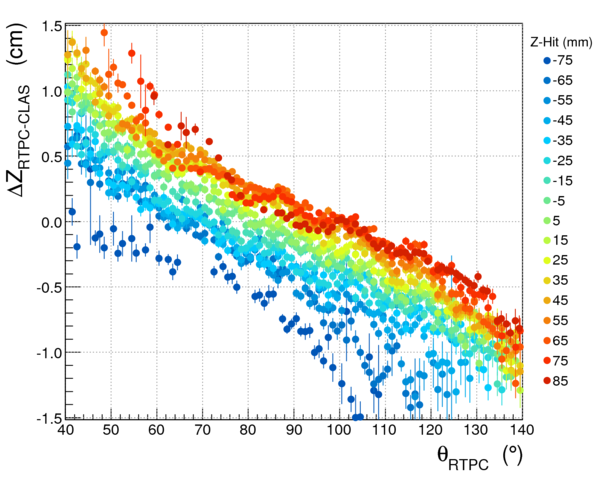
\includegraphics[width=0.49\textwidth]{pics/dz_theta_zhit_fid_A_small.png}
    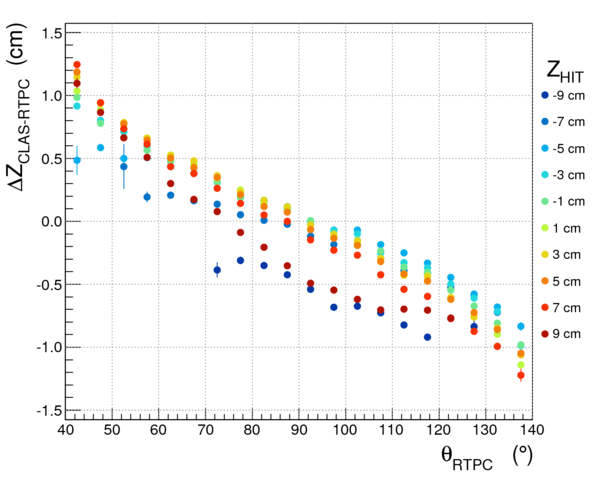
\includegraphics[width=0.49\textwidth]{pics/dz_theta_zhit_afterzcorr_small.png}
    \caption{The effect of a $z$-dependent correction derived from 90$^\circ$ tracks in Sec. \ref{sec:90deg}: before (left), and after (right) correction.\label{fig:dz_theta_z_corr}}
%    . The uncorrected $z$-dependence (left) is largely removed (right) except for tracks that cross near the ends of the drift region, while the $\frac{1}{\tan\theta}$ angular dependence is unaffected.\label{fig:dz_theta_z_corr}}
\end{figure}

%\begin{figure}[htbp]\centering
%    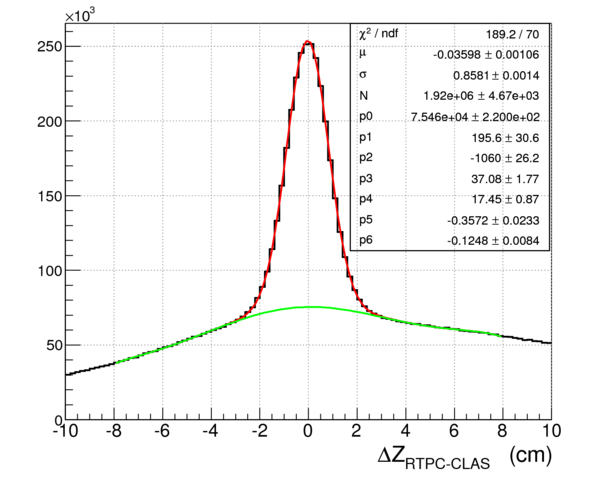
\includegraphics[width=8cm]{pics/dvzRTPC-CLAS_small.png}
%    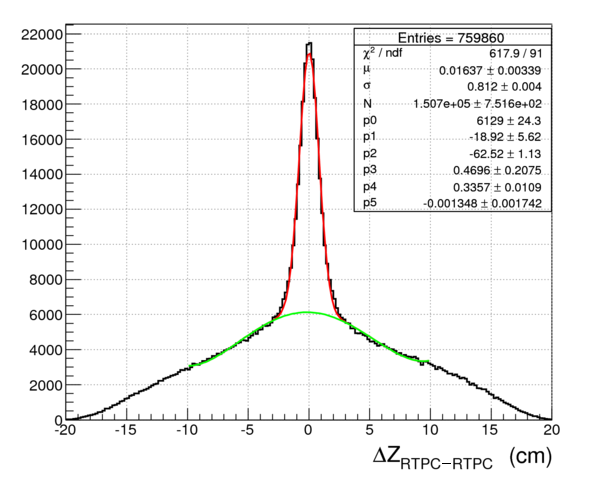
\includegraphics[width=8cm]{pics/dvzRTPC-RTPC_small.png}
%    \caption{The RTPC-CLAS (left) and RTPC-RTPC (right) $z$-vertex differences for two tracks in the same event.\label{fig:dzclasrtpc1d}}
%\end{figure}

\section{Effect of Incorrect Radial Drift Speed}
Based upon some old MAGBOLTZ studies by BoNuS, the radial drift speed varies by a factor of 2 from cathode to GEMs.   We can estimate the effect of an error on speed with some simple geometry and straight tracks.

First, assume the radial drift speed near the GEMs (large radius) is accurate or insignificant, since the drift path is very small here.  Next, {\it assume a relative error on the speed that increases linearly with distance from the GEMs}:
\begin{equation}
    \frac{\delta v}{v}=k\frac{\rho_g-\rho}{r}.
    \label{eq:dvoverv}
\end{equation}
The radial position of the tracking point is $\rho$, the GEMs are at a radius of $\rho_g$, and the radial thickness of the drift region is $r$.  The relative error on the speed at the cathode is then $k$ in this scenario.

This error on radial drift speed will create a proportional error on the radial position of the reconstructed track points,
\begin{equation}
    \frac{\delta\rho}{\rho}=\frac{\delta v}{v}.
    \label{}
\end{equation}
However, we should estimate using the average error on the speed the drift electrons will experience.  This can be estimated by using the halfway point between the track position and the GEMs:
\begin{equation}
    \frac{\delta\rho}{\rho}=k\frac{\rho_g-\rho}{2r}.
    \label{}
\end{equation}
At the cathode, since $\rho_g=2\rho_c$ in our RTPC, this becomes $\delta\rho=k\rho_c/2$.
Since the measured radial position near the GEMs is assumed accurate, we can estimate the error on the angle with just the error on the radial position near the cathode:
\begin{equation}
    \delta\theta = \frac{\partial\theta}{\partial\rho}\delta\rho_c=\left[\frac{\cos\theta\sin\theta}{r}\right]\left[\frac{k\rho_c}{2}\right]=\frac{k}{2}\cos\theta\sin\theta
    \label{}
\end{equation}
And converting this into the resulting error on $z$-vertex:
\begin{equation}
    \delta z_v=\frac{\partial z}{\partial\theta}\delta\theta=\frac{k\mathcal{R}}{2\tan\theta}
    \label{}
\end{equation}

So, based upon this very simple estimate, a $z$-independent {\it error in the radial drift speed that increases with distance from the GEMs} will (1) {\it have a} $\frac{1}{\tan\theta}$ {\it effect on $z_v$ similar to a pad pitch error and the shape seen in the real data}, (2) of course not create an error on $z_v$ for tracks at 90$^\circ$, and (3) of course not create a $z$-dependence.

If we assume that pad pitch and drift speed errors can be simply added and that the pad pitch error is 5.5\% from the previous section, then the $\theta$-dependence can be fit again to derive a drift speed error.  With all these assumptions, this suggests a $\sim$15\% error on radial drift speed at the cathode could account for the measured errors on the $z$-vertex.

\section{Reconstructed Track Points}
The previous studies with real data all used the results of a helix fit to all the track hits in the RTPC.  We can also look at individual tracking points.  While this will not provide the precision of a helix fit, it may give clues to help isolate the source of the problem.
We do have the reconstructed positions of the first (nearest the cathode) and last (nearest the GEMs) points of deposited charge recorded in the {\texttt GCPB} bank for each track.  In the following figures they are referred to by the suffixes ``CAT'' (first) and ``GEM'' (last).
\subsection{Helix Fit Versus Straight Line}
Unless there is a systematic problem in the helix fit itself, for straight tracks the result from the helix fit and the polar angle calculated from a straight line between the first and last hits ($\theta_{CAT-GEM}$) should agree.  Figure \ref{fig:catgemhel}, with $p/q>$250 MeV, shows they do to within a small fraction of a degree over all angles.  This is much too small to correlate with the $z$-vertex errors shown previously for highest momentum tracks where the $\theta$-dependence was largest (see Fig. \ref{fig:dz_mom}).
\begin{figure}[htbp]\centering
    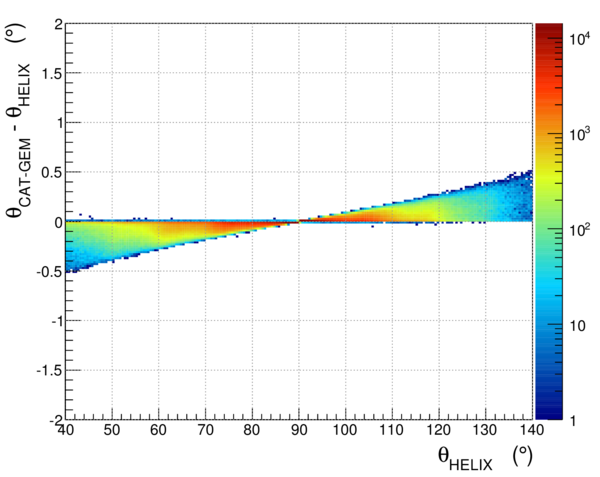
\includegraphics[width=0.5\textwidth]{pics/dtheta_theta_catgem-helix_poverq_gt_250_small.png}
    \caption{The difference between the polar angle calculated from the helix and from a straight line between the first and last measured track hits.  Note the logarithmic color scale. Only tracks with a reconstructed $p/q>250$ MeV are shown, creating the appearance of a diagonal cut.\label{fig:catgemhel}}
\end{figure}
\subsection{One Tracking Point with Electron Reference}
We can now use only one tracking point from these ``straight'' tracks if we have another reference.  For this we can use the electron's $z$-vertex.
%after requiring concidence between the electron and RTPC track (see top left of Fig. \ref{fig:dzclasrtpc}).
It is expected that the first tracking point near the cathode should have worse precision than the last one near the GEM due to the large difference in drift path length.
But if they are reconstructed with similar accuracy, we should see same trend in both.%then the trend of the peak position in the two plots should be the same.  

The difference between the polar angle of the helix fit and that calculated from a straight line between the electron's $z$-vertex and one of the RTPC tracking points is shown in Fig. \ref{fig:dthetacatgem}.
The oscillation for the point near the GEMs relative to the helix fit (left panel) has a very similar magnitude as Fig. \ref{fig:dtheta1} (which was calculated from the $z$-vertex error reconstructed from the helix fit assuming the fit's angle was at fault).  This is consistent with the point near the GEM being more accurate than the helix fit as a whole.  And the point near the cathode shows significantly larger angular dependence in the right panel of Fig. \ref{fig:dthetacatgem}, consistent with a drift path effect.

%:  for the last tracking point, the difference varies from -5$^\circ$ to +7$^\circ$, while for the first tracking point it varies from -8$^\circ$ to +14$^\circ$.

\begin{figure}[htbp]\centering
    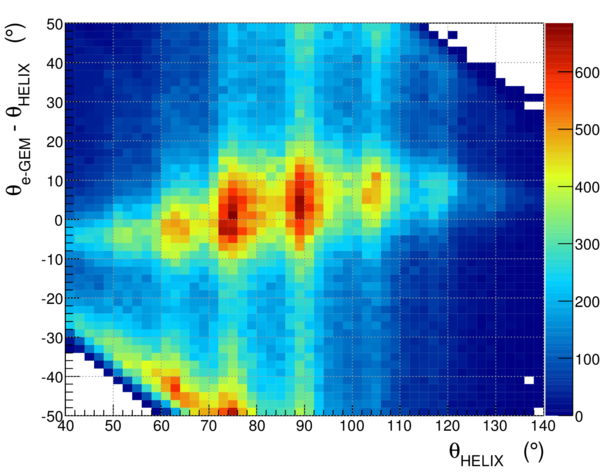
\includegraphics[width=0.49\textwidth]{pics/dtheta_theta_elgem-helix_poverq250.png}
    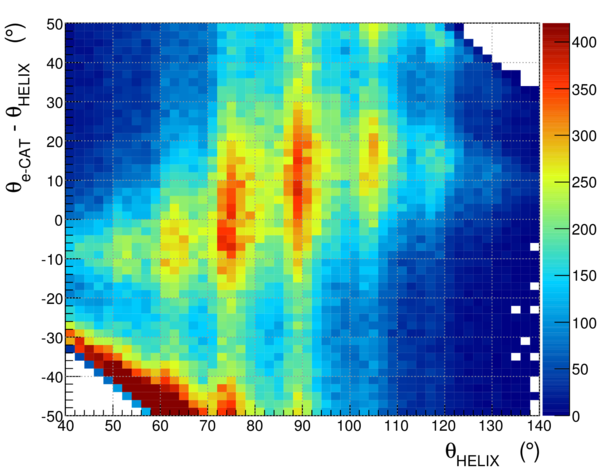
\includegraphics[width=0.49\textwidth]{pics/dtheta_theta_elcat-helix_poverq250.png}
    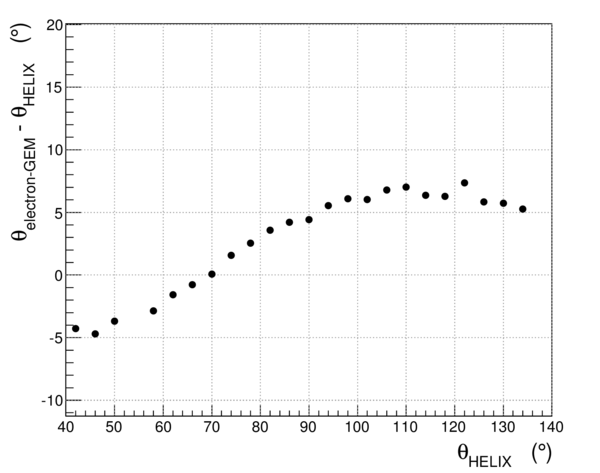
\includegraphics[width=0.49\textwidth]{pics/dtheta_theta_elgem-helix_poverq_gt_250_FIT_small2.png}
    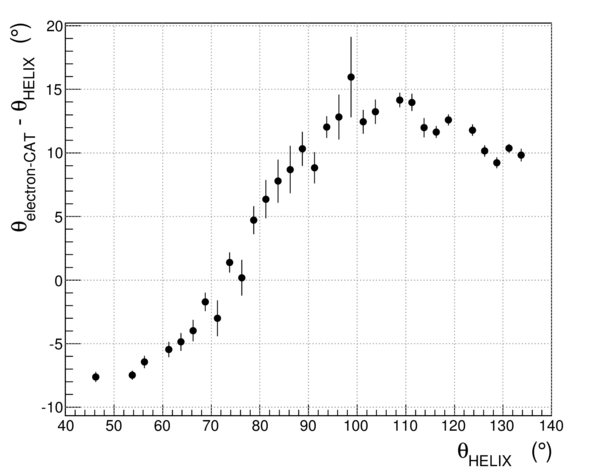
\includegraphics[width=0.49\textwidth]{pics/dtheta_theta_elcat-helix_poverq_gt_250_FIT_small.png}
    \caption{As a function of track angle, the difference between the track angle calculated from the helix fit and that calculated from the electron vertex and the last (left) and first (right) point in the helix fit.  Only ``straight'' tracks with measured $p/q>250$ MeV are shown.  The bottom row is the peak position.\label{fig:dthetacatgem}}
\end{figure}


\section{Conclusion}
Misalignment, energy loss, magnetic field error, and time-dependence of calibration all seem to be unlikely causes.  A full simulation could be helpful for isolating the cause.
The source of the error could be a combination of factors.

Open possibilities include, but are not limited to, \sout{an error on the pad pitch} (which would have the linear $z$-dependence and $\frac{1}{\tan\theta}$ dependence found in the data), unaccounted for effects in the radial drift path speed (which are shown capable of creating the $\frac{1}{\tan\theta}$ shape and would become largest near the ends of the RTPC), some unstudied effect of division of the charge into a discrete number of pads.
\subsection{Pad Pitch}
After this study, the pad pitch of a duplicate EG6 GEM was measured on September 6, 2013 with a micrometer by averaging over all pads in each direction, $\hat{\phi}$ and $\hat{z}$.   The result was within 0.1\% of the nominal value used in the the reconstruction code in both cases.  Based upon that measurement, it is very unlikely the effects we are seeing are due to incorrect pad pitch.

%Is there some effect in the drift paths that can be angle-dependent, even near the center of the solenoid field?  How far from the nominal value can the pad pitch really be?
\appendix
\section{Track Quality}
Two track reconstruction quality variables are noticed to have significant dependence on polar angle in Fig. \ref{fig:sdist}.  The $\chi^2$ of the helix fit is always good for $\theta\sim90^\circ$, but increases roughly symmetrically as the angle departs from 90$^\circ$.  The variable {\texttt sdist} is the distance along the helix from the cathode to the point on the helix that is closest to the first deposited charge in the track.  It should ideally be narrowly peaked around zero (and it is near 90$^
\circ$), but broadens and heads negative as the track angle departs from 90$^\circ$.
\begin{figure}[htbp]\centering
    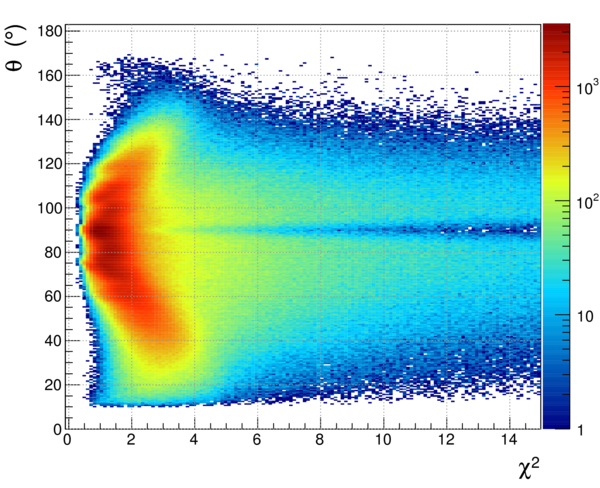
\includegraphics[width=0.49\textwidth]{pics/chi2_vs_theta_small.png}
    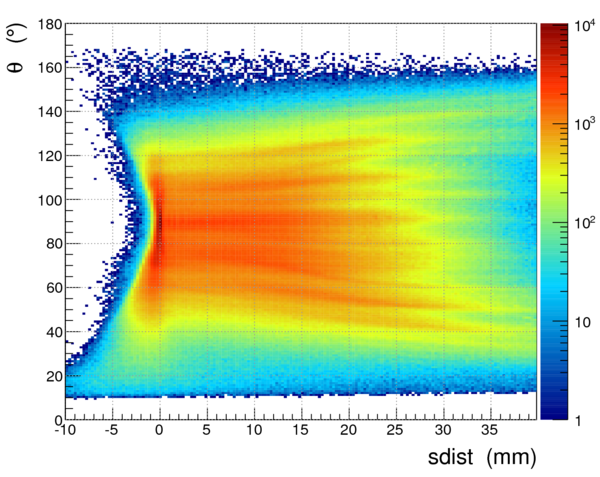
\includegraphics[width=0.49\textwidth]{pics/sdist_vs_theta_small.png}
    \caption{The angular dependence of the helix fit's $\chi^2$ (left) and {\texttt sdist} (right). 
    \label{fig:sdist}}
\end{figure}


%\bibliography{padpitch}
\end{document}









\begin{comment}
For the simplest case, consider tracks reconstructed with angles very near $90^\circ$.  The expected error on the reconstructed vertex due to an error on the pad pitch, $\delta p$, depends on the number of pads, $n$, the track is from $Z_0$ and can be written as
\begin{equation}
    \delta z_v^{90^{\circ}}\ =\ n\delta p\ =\ \frac{z_v-Z_0}{p}\delta p.
    \label{eq:dz90}
\end{equation}
It is linear in $z_v$ and proportional to the relative error on the pad pitch.  The error is zero at $Z_0$, where the two pad configurations (the real one and the one used in the reconstruction code) coincide.
Another special case that allows for simple analysis is when the vertex of the RTPC track is near where the real GEM pad coincides with that used for reconstruction, $Z_0$.  The relationship between vertex and pad pitch is more complicated than at 90$^\circ$ due to an additional error on $\theta$ that does not exist at 90$^\circ$:
\begin{equation}
    \delta z_v^{Z_0}\ =\ \frac{\partial z_v}{\partial p}\delta p\ +\ \frac{\partial z_v}{\partial \theta}\frac{\partial\theta}{\partial l}\frac{\partial l}{\partial p}\delta p
%    \delta z_v^{Z_0}\ =\ \frac{\partial z}{\partial p}\biggr|_{Z_0}\delta p\ +\ \frac{\partial z}{\partial \theta}\frac{\partial\theta}{\partial p}\delta p
%    \delta z_v^{Z_0} = (z_d-Z_0)\frac{\delta p}{p}\ +\ A
    \label{eq:dzZ0}
\end{equation}
The first term in Eq. \ref{eq:dzZ0} is the same $z$-dependent shift as for the 90$^\circ$ case except that $z_v$ is replaced by the angle-dependent $z_d$, the position of the track in the middle of the drift region:
\begin{equation}
    \frac{\partial z_v}{\partial p}\ =\ \frac{z_d-Z_0}{p}\ =\ \frac{z_v-Z_0+R/\tan\theta}{p}
    %\frac{\partial z}{\partial p}\biggr|_{Z_0}\ =\ \frac{v_d-Z_0}{p}\ =\ \frac{v_z-Z_0+R/\tan\theta}{p}
    \label{}
\end{equation}
%That reduces to Eq. \ref{eq:dz90} at 90$^\circ$.
The second term in Eq. \ref{eq:dzZ0} is due to a (de)compression in $l$ (see Fig. \ref{fig:diagram}) that is independent of the longitudinal position, and using $l=np$:
\begin{equation}
    \frac{\partial z_v}{\partial\theta} = \frac{R}{\sin^2\theta}\ \ \ \ \ \ \ \ \  
    \frac{\partial\theta}{\partial l} = \frac{\sin^2\theta}{r}\ \ \ \ \ \ \ \ \ 
    \frac{\partial l}{\partial p} = n
\end{equation}
\end{comment}
